\Chapter{Tesztelés}

\Section{Telepítés és használat}

\Section{Használati útmutató}
Első lépésként felhasználói fiók létrehozása szükséges. A regisztráció során a felhasználónak meg kell adnia egy egyedi, még nem használatban lévő felhasználónevet és egy legalább nyolc karakterből álló jelszót, ezt követően igénybe veheti a weboldal szolgáltatásait.

Ha a felhasználó már rendelkezik saját fiókkal, akkor a bejelentkezés után érheti el az alkalmazás funkcióit.
A bejelentkezést követően a felhasználó hozzáférést kap a saját sémáihoz, amelyek kezelésére külön menüpont áll rendelkezésre.

\begin{figure}[h]
\centering
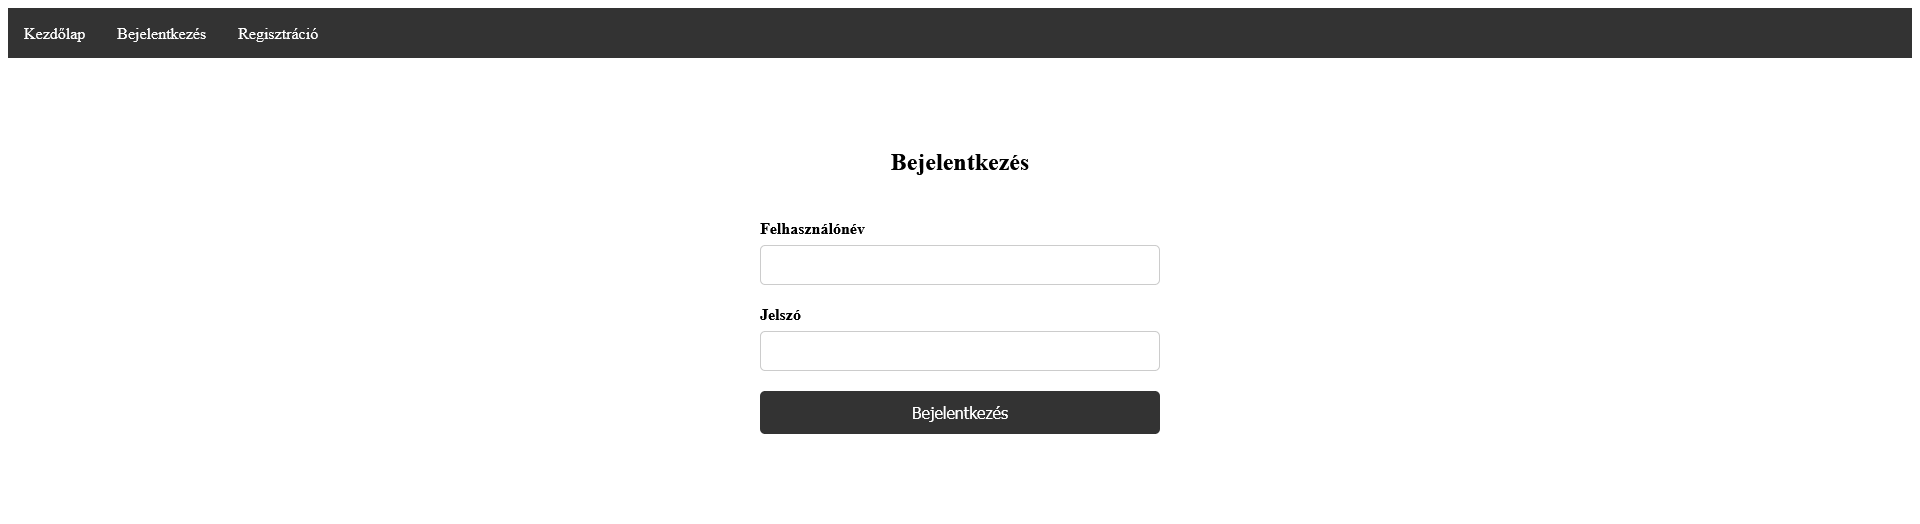
\includegraphics[scale=0.3]{images/bejelentkezes.png}
\caption{A bejelentkezési felület.}
\label{fig:bejelentkezes}
\end{figure}

A Sémák menüpontban a felhasználó megtekintheti a korábban létrehozott sémáit, valamint új sémát is feltölthet. A listában megjelennek az egyes sémákhoz tartozó alapvető információk és a kezelésükhöz szükséges műveletek. A felhasználónak lehetősége van a sémák adatainak módosítására, a hozzájuk tartozó kitöltött űrlapok megtekintésére, illetve a sémák törlésére.

\begin{figure}[h]
\centering
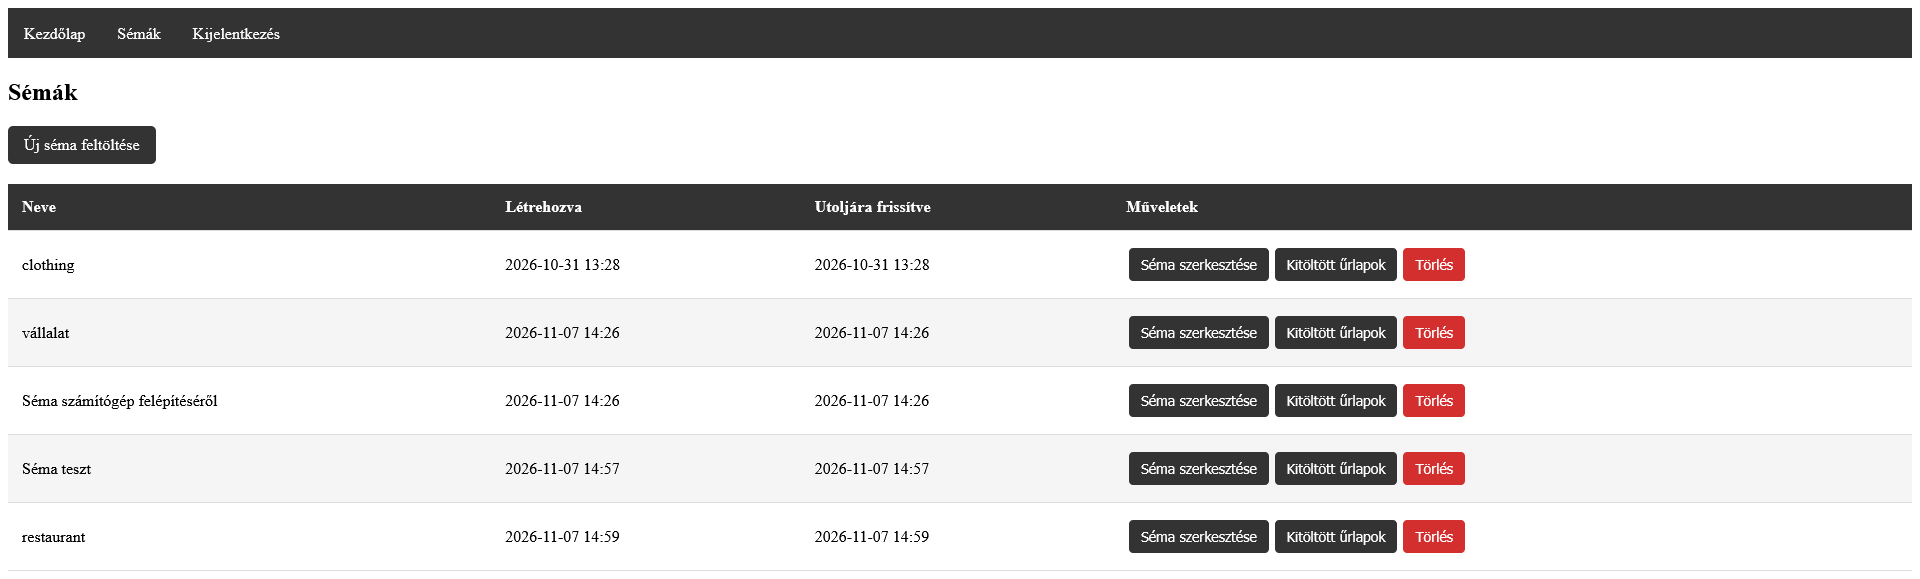
\includegraphics[scale=0.3]{images/semaLista.png}
\caption{A séma oldal.}
\label{fig:semaLista}
\end{figure}

Ha új sémát akar feltölteni a felhasználó azt megteheti az új séma feltöltése gombra kattintva. A felhasználónak elsőként meg kell adnia a létrehozandó űrlap nevét, majd hozzá kell rendelnie az űrlap szerkezetét meghatározó XML-sémát. A séma megadása kétféleképpen történhet: a felhasználó közvetlenül beillesztheti vagy begépelheti az XSD-kódot a szöveges mezőbe, illetve feltölthet egy korábban elkészített XSD-fájlt. Ezt követően a séma feltöltés gombbal menthető az új séma és a felhasználó megkapja a linket amin az űrlap elérhető.

\begin{figure}[h]
\centering
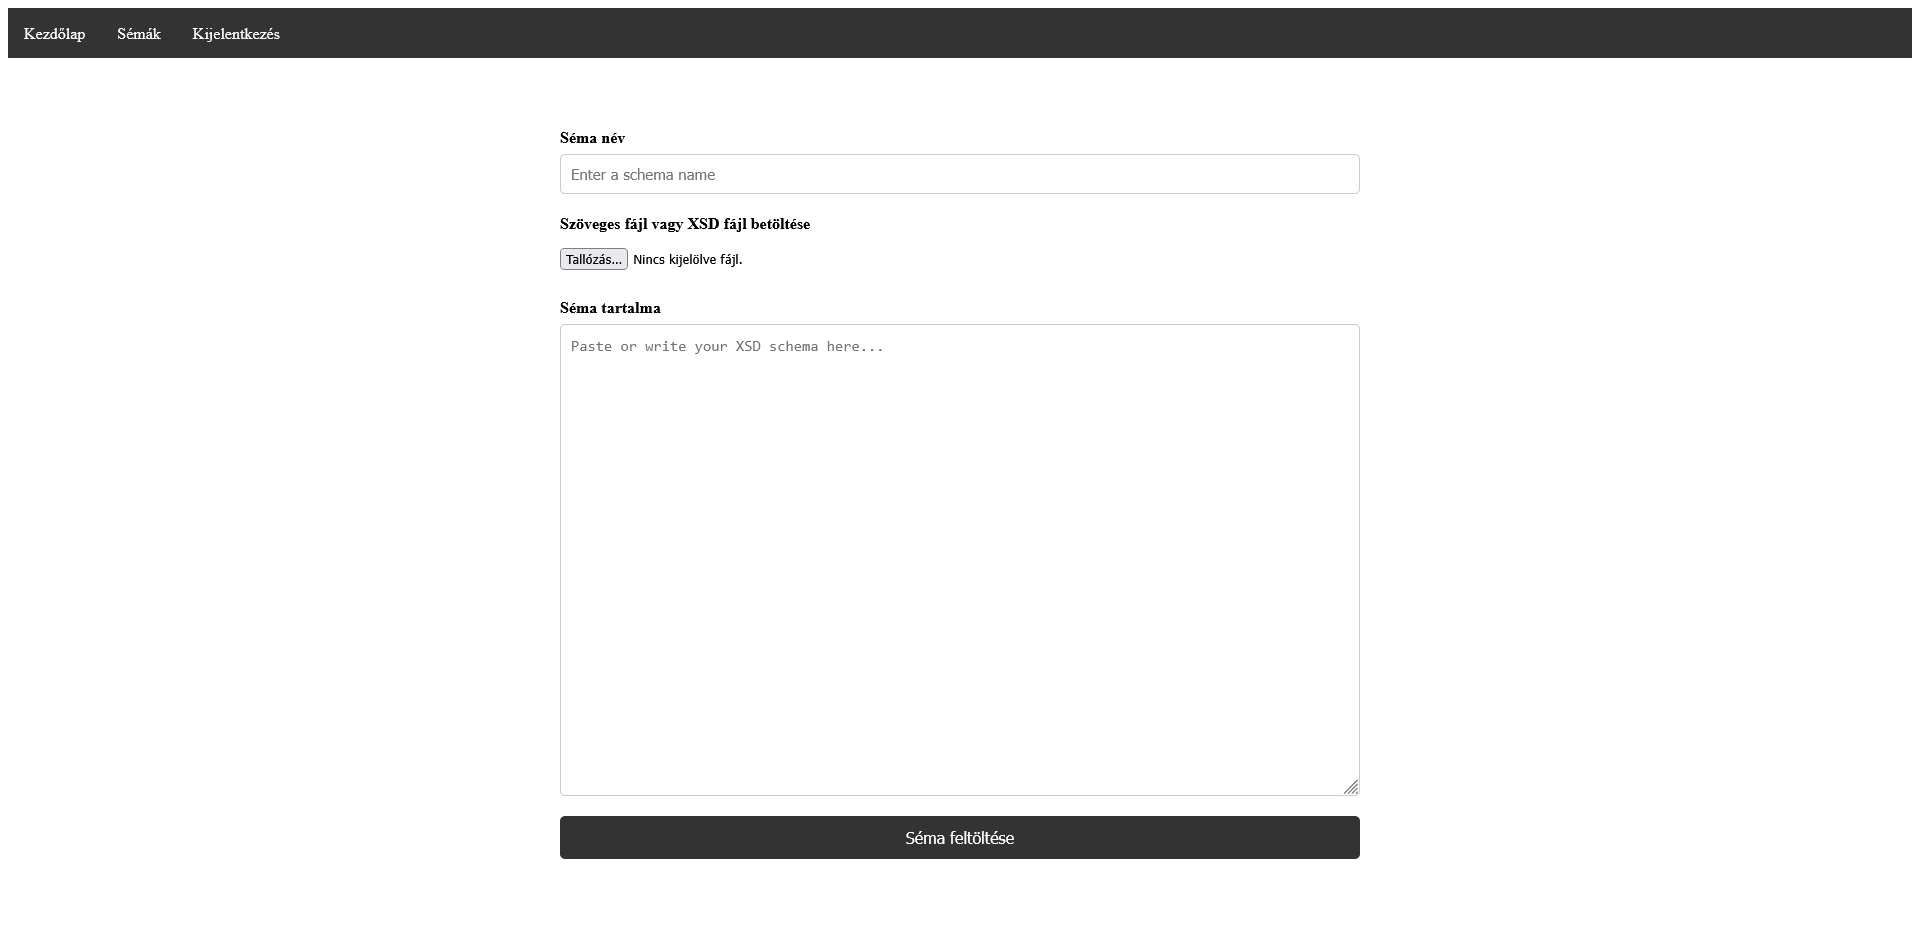
\includegraphics[scale=0.3]{images/semaFeltoltes.png}
\caption{A séma feltöltésének oldal.}
\label{fig:semaFeltolt}
\end{figure}
A lementett sémákat feltöltés után a séma szerkesztése gombra kattintva lehetséges módosítani. Ezen felületen meg lehet változtatni a megadott nevet, az XSD-kódot, megtekinthető az űrlap linkje, és helyben legenerálható az űrlap. Az itt megtalálható űrlap kitöltés után nem lesz elmentve, hanem egy XML kódot készít, ezzel a felhasználó biztosíthatja, hogy megfelelő eredményeket kapjon.

A létrehozott sémákhoz az alkalmazás külön elérési hivatkozást biztosít. Ezen keresztül a felhasználók megnyithatják az adott XML-séma alapján automatikusan generált űrlapot. Az űrlap megjelenése és felépítése a hozzá rendelt XSD-sémától függ. A séma határozza meg az űrlap elemeit, azok típusát, kötelező vagy opcionális jellegét, valamint az értékkorlátozásokat. Az alkalmazás a séma feldolgozása során a meghatározott elemekhez megfelelő beviteli mezőket rendel. Egyszerű szöveges értékek esetén szövegmezők, számértékek esetén numerikus beviteli mezők, felsorolások esetén legördülő listát jelenhetnek meg.

Az alkalmazás lehetőséget biztosít arra is, hogy a felhasználó az XSD-sémában további információkat adjon meg a generált űrlap megjelenésével kapcsolatban. Erre az xs:annotation és xs:appinfo szerkezetek használhatók. Az elemhez tartozó űrlapkomponens típusa az xs:appinfo részen belül adható meg. A lenti példában a radio érték hatására a mező legördülő lista helyett rádiógombokként jelenik meg. Az űrlap bemeneti felületeihez leírás is rendelhető az xs:description segítségével. Ebben megadható, hogy milyen választ várunk a felhasználótól, illetve milyen formai követelményeknek kell megfelelnie a megadott értéknek. 
\begin{java}
majd talalnom kell xml-t
<xs:element name="speed" type="speedType">
 <xs:annotation>
  <xs:appinfo>
   <xs:type>radio</xs:type>
   <xs:description>How fast would you rate the speed of delivery
   <xs:description>
  </xs:appinfo>
 </xs:annotation>
</xs:element>
\end{java}
Az következő bemeneti elemeket támogatja a program amik az xs:appinfo-n belül megadhattóak:
\begin{itemize}
\item date
\item select
\item radio
\item checkbox
\item number
\item range
\item text
\item textarea
\item password
\item email
\end{itemize}

Az alkalmazás jelenleg nem támogatja az XSD-szabvány bizonyos szerkezeteinek teljes körű feldolgozását. Ezek használata esetén megtörténhet, hogy a generált űrlap nem képes az összes séma által meghatározott feltétel érvényesítésére, így a létrehozott XML-dokumentum nem fog megfelelni az eredeti sémának.

A jelenleg korlátozottan vagy egyáltalán nem támogatott szerkezetek a következők:
\begin{itemize}
\item list
\item unio
\item choice
\item extend
\end{itemize}
Az xs:union használata esetén az alkalmazás egyszerű szöveges beviteli mezőt jelenít meg, azonban nem végzi el az egyes tagtípusoknak megfelelő értékellenőrzést.

Az xs:list szerkezetek feldolgozása korlátozott: az alkalmazás az egyszerű beépített típusok esetében képes kezelni a listaelemeket, azonban egyedi típus megadása esetén az azokhoz tartozó korlátozásokat nem érvényesíti.

Az xs:choice szerkezeteket az alkalmazás nem kezeli különálló választási lehetőségként, hanem a többi komplex elemhez hasonlóan dolgozza fel. Ennek következtében nem biztosított, hogy a generált XML-dokumentum megfeleljen az eredeti séma által meghatározott választási feltételeknek.

Az xs:extension segítségével megadott típusbővítéseket az alkalmazás nem dolgozza fel, ezért az örökölt szerkezeti elemek és korlátozások nem feltétlenül jelennek meg a generált űrlapon.

\begin{figure}[h]
\centering
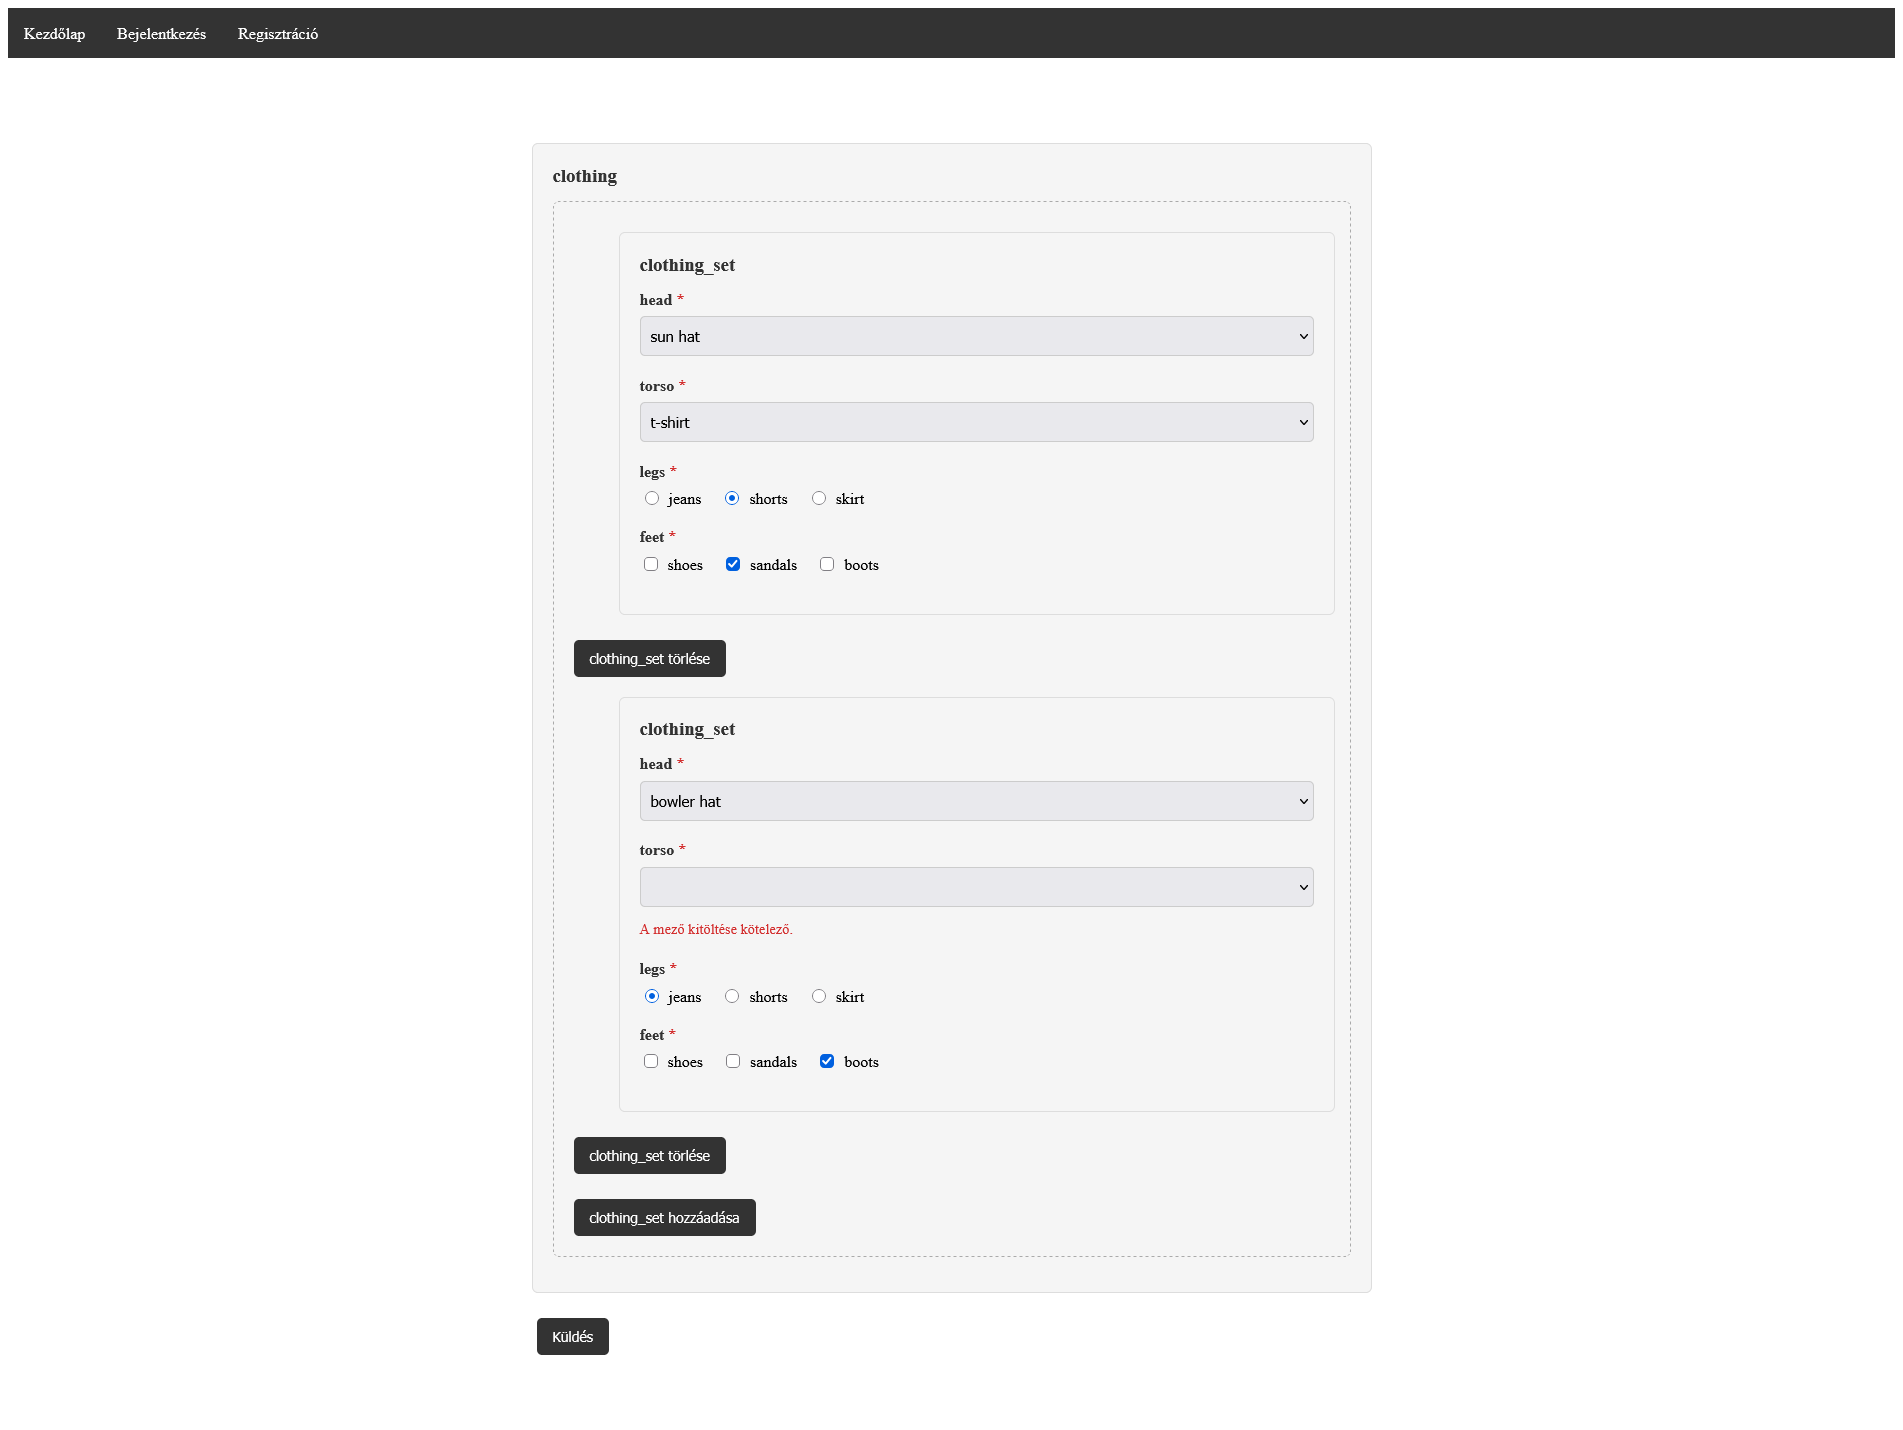
\includegraphics[scale=0.3]{images/urlapKitoltes.png}
\caption{Egy generált űrlap.}
\label{fig:urlapKitolt}
\end{figure}

A beküldött adatok a megfelelő séma adatlapján található kitöltött űrlapok menüpontban tekinthetők meg. Itt a felhasználó áttekintheti az adott sémához tartozó beküldéseket. A beküldött űrlapok listájában megjelennek a kapcsolódó információk, például a beküldés időpontja és a beküldő felhasználó neve, amennyiben az rendelkezésre áll.

Minden beküldött űrlaphoz tartozik egy XML-dokumentum, amely az űrlap kitöltése során megadott adatokat tartalmazza. A dokumentum letöltésével az adatok az alkalmazástól függetlenül is felhasználhatók, illetve további feldolgozásra átadhatók.

\begin{figure}[h]
\centering
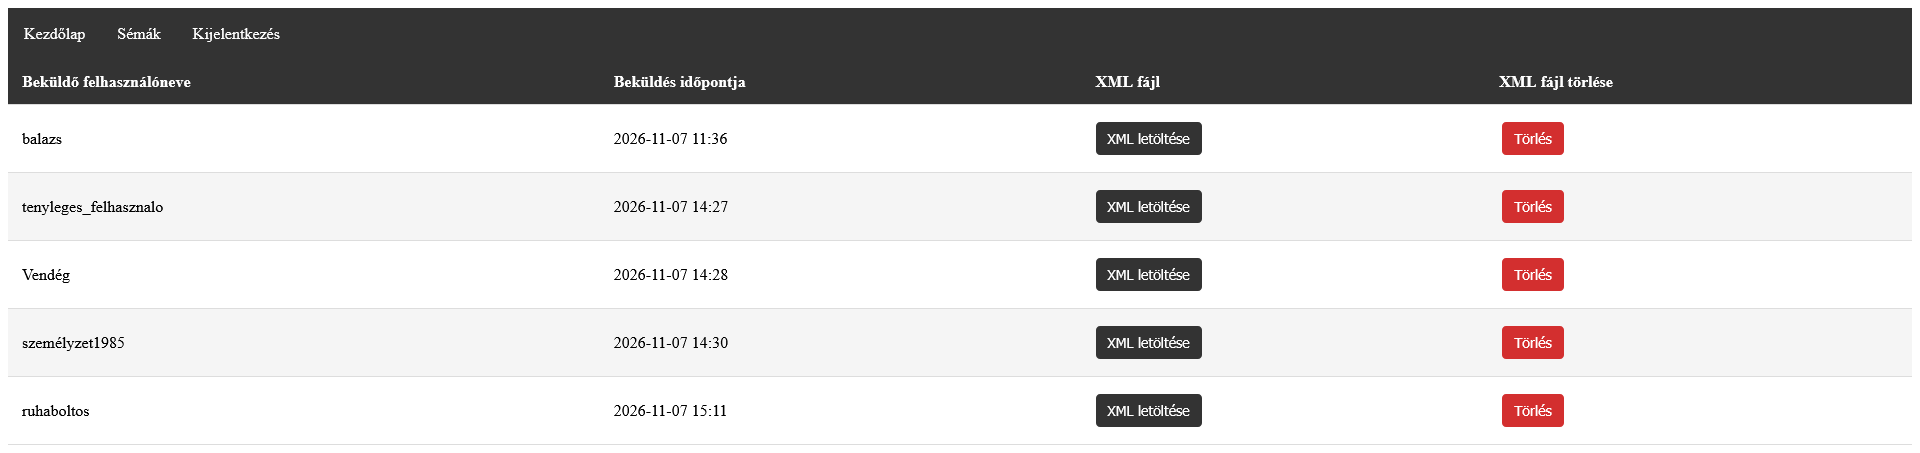
\includegraphics[scale=0.3]{images/kitoltottUrlapok.png}
\caption{Kitöltött űrlapok listája egy sémához.}
\label{fig:kitoltottUrlapok}
\end{figure}

\section{Tesztelési lehetőségek}
